\documentclass[draft]{lipics-v2021}

\bibliographystyle{plainurl}

\title{Engineering a Planar Convex Hull Algorithm}

\author{Thomas Koopman}{Radboud University, the Netherlands}{thomas.koopman@ru.nl}{https://orcid.org/0009-0001-1031-7226}{}

\author{Jordy Aaldering}{Radboud University, the Netherlands}{jordy.aaldering@ru.nl}{https://orcid.org/0009-0001-3018-5152}{}

\author{Bernard van Gastel}{Radboud University, the Netherlands}{bernard.vangastel@ru.nl}{https://orcid.org/0000-0002-0974-4634}{}

\authorrunning{T.J. Koopman, J. Aaldering, B. van Gastel} %TODO mandatory. First: Use abbreviated first/middle names. Second (only in severe cases): Use first author plus 'et al.'

\Copyright{Thomas Koopman, Jordy Aaldering, Bernard van Gastel} %TODO mandatory, please use full first names. LIPIcs license is "CC-BY";  http://creativecommons.org/licenses/by/3.0/

\ccsdesc[100]{\textcolor{red}{Replace ccsdesc macro with valid one}} %TODO mandatory: Please choose ACM 2012 classifications from https://dl.acm.org/ccs/ccs_flat.cfm 

\keywords{Dummy keyword}

%\relatedversion{} %optional, e.g. full version hosted on arXiv, HAL, or other respository/website
%\relatedversiondetails[linktext={opt. text shown instead of the URL}, cite=DBLP:books/mk/GrayR93]{Classification (e.g. Full Version, Extended Version, Previous Version}{URL to related version} %linktext and cite are optional

%\supplement{}%optional, e.g. related research data, source code, ... hosted on a repository like zenodo, figshare, GitHub, ...
%\supplementdetails[linktext={opt. text shown instead of the URL}, cite=DBLP:books/mk/GrayR93, subcategory={Description, Subcategory}, swhid={Software Heritage Identifier}]{General Classification (e.g. Software, Dataset, Model, ...)}{URL to related version} %linktext, cite, and subcategory are optional

%\acknowledgements{I want to thank \dots}%optional

\usepackage{algorithm}
\usepackage{algorithmicx}
\usepackage[noend]{algpseudocode}
\usepackage{amsmath}
\usepackage{amsthm}
\usepackage{amssymb}
\usepackage{calculator}
\usepackage{calc}
\usepackage{graphicx}
\usepackage{listings}
\usepackage{hyperref}
\usepackage{pgfplotstable}
\usepackage{siunitx}
\usepackage{tikz}
\usetikzlibrary{graphs}
\usetikzlibrary{quotes}
\usetikzlibrary{decorations.pathreplacing}
\usepackage{xcolor}

\renewcommand{\algorithmicrequire}{\textbf{Input:}}
\renewcommand{\algorithmicensure}{\textbf{Output:}}
\newcommand{\glasgowcomment}[2]{{\textbf #1: }{\textrm \textsf #2}}
\newcommand{\tkcomment}[1]{\glasgowcomment{TK}{\color{orange} #1}}
\DeclareMathOperator*{\argmax}{argmax}
\DeclareMathOperator*{\argmin}{argmin}

\pgfplotstableset{col sep = comma, fixed zerofill, precision=3, fixed}
\sisetup{exponent-mode = fixed, fixed-exponent=0,
         round-mode = figures, round-precision = 2}

\begin{document}

\maketitle

\begin{abstract}
    \tkcomment{TODO}
%    Finding the convex hull is a fundamental problem in computational geometry.
%    
%    A well-rounded and fast algorithm is Quickhull, a problem similar to 
%    Quicksort.
%
%    In this paper, we take a thorough look at implementing this algorithm,
%    investigating runtime, memory-usage, energy consumption, and 
%    numerical accuracy.
%
%    We also provide a novel parallel algorithm.
%
%    This results in a runtime improvement of up to $13 \times$ for a
%    sequential implementation, and up to $? \times$ for a multithreaded
%    implementation. 
\end{abstract}


\section{Introduction}

The convex hull of a set of points in $\mathbb{R}^2$, can be intuitively 
understood as follows: Put a nail in a piece of wood at each point. Then span 
an elastic band around these nails. The resulting polygon is the convex hull of 
the points.

This is a fundamental algorithm in Computational Geometry with applications
in .... 

To be more precise, a convex combination of points $x_1, \cdots, x_n$ is a 
weighted average $\lambda_1 \cdot x_1 + \cdots \lambda_n \cdot x_n$, 
$\lambda_i \geq 0, \sum_{i = 1}^n \lambda_i = 1$. A set that is closed under
taking convex combinations is called convex. The convex hull of a set $X$ is
the set of all its convex combinations and denoted with $CH(X)$. For $X$
a finite set, the convex hull is a polygon with vertices in $X$.

A polygon is determined by its vertices and edges, which we can efficiently
store by listing the vertices in (counter-)clockwise order. The edges are given 
by adjacent vertices.

Computing this list is the convex hull problem. There exist many algorithms for 
this \cite{}, of which we find Quickhull to be the fastest (see
Section~\ref{sec:perf}). This algorithm resembles Quicksort in that
it recursively splits the points into two sets. Unlike Quicksort however,
more points than just the pivot may be discarded. Moreover, we are not
free to choose the pivot, which turns out to make parallelisation challenging.
Nonetheless, we can adept recent insights from the sorting community to engineer
a fast Quickhull implementation for shared memory computers.

We make the following contributions.

\begin{itemize}
    \item We present a vectorized algorithm for extracting two disjoint
          subsets in-place.
    \item We parallelise this algorithm in a bandwidth-friendly manner.
    \item We evaluate the performance on two different platforms. 
\end{itemize}


\section{Preliminaries}

\subsection{Quickhull}

The Quickhull algorithm makes use of two important facts 
illustrated by Figure~\ref{fig:quickhull}. First, if $p$, $q$ are in the 
convex hull, then any point $u$ with maximum distance to the line $\vec{pq}$, 
is in the convex hull as well. Secondly, any point within the triangle 
$puq$ is not in the convex hull. Only the points to the left of $pu$ and 
to the right of $uq$ still need to be considered.

\begin{figure}[ht]
    \begin{subfigure}{0.45\textwidth}
    % Generated with 20 points, width 5, height 8
    \resizebox{\columnwidth}{!}{%
        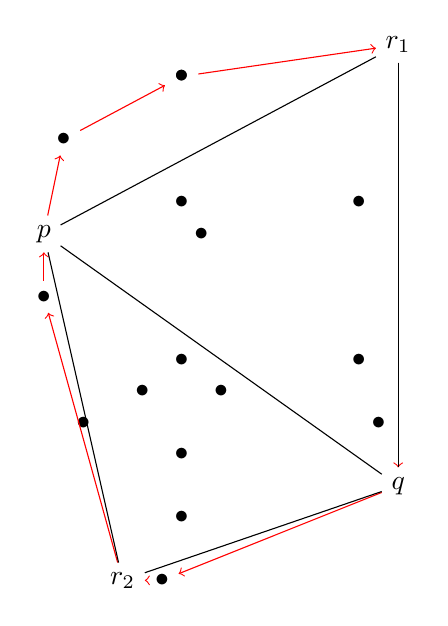
\begin{tikzpicture}
            \node (6_2) at (1.500, 0.800) {$\bullet$};
            \node (16_9) at (4.000, 3.600) {$\bullet$};
            \node (7_9) at (1.750, 3.600) {$\bullet$};
            \node (7_18) at (1.750, 7.200) {$\bullet$};
            \node (9_8) at (2.250, 3.200) {$\bullet$};
            \node (16_14) at (4.000, 5.600) {$\bullet$};
            \node (p) at (0.000, 5.200) {$p$};
            \node (2_7) at (0.500, 2.800) {$\bullet$};
            \node (r2) at (1.000, 0.800) {$r_2$};
            \node (7_14) at (1.750, 5.600) {$\bullet$};
            \node (8_13) at (2.000, 5.200) {$\bullet$};
            \node (0_11) at (0.000, 4.400) {$\bullet$};
            \node (r1) at (4.500, 7.600) {$r_1$};
            \node (7_6) at (1.750, 2.400) {$\bullet$};
            \node (q) at (4.500, 2.000) {$q$};
            \node (1_16) at (0.250, 6.400) {$\bullet$};
            \node (7_18) at (1.750, 7.200) {$\bullet$};
            \node (17_7) at (4.250, 2.800) {$\bullet$};
            \node (7_4) at (1.750, 1.600) {$\bullet$};
            \node (5_8) at (1.250, 3.200) {$\bullet$};

            \graph {(0_11) ->[red] (p)};
            \graph {(p) ->[red] (1_16)};
            \graph {(1_16) ->[red] (7_18)};
            \graph {(7_18) ->[red] (r1)};
            \graph {(r1) ->[red] (q)};
            \graph {(q) ->[red] (6_2)};
            \graph {(6_2) ->[red] (r2)};
            \graph {(r2) ->[red] (0_11)};
            \graph {(p) --[black] (q)};
            \graph {(p) --[black] (r1)};
            \graph {(r1) --[black] (q)};
            \graph {(q) --[black] (r2)};
            \graph {(r2) --[black] (p)};
        \end{tikzpicture}
    }
    \caption{The points $p$ and $q$ are the left-most and 
             right-most points, and therefore in the hull. The points $r_1$,
             $r_2$ are furthest from the line $pq$, and also in the hull. Any
             point within the two triangles cannot be in the convex hull.}
    \label{fig:quickhull}
    \end{subfigure}
    \hfill
    \begin{subfigure}{0.45\textwidth}
    \begin{algorithmic}[1]
        \Require $P: $ set of points in $\mathbb{R}^2$
        \Ensure $H: $ vertices of convex hull of $P$ in clockwise order.
        \State Let $p$ be the left-most point
        \State Let $q$ the right-most point
        \State $S_1 := \{u \in P \ | \ clockwise(p, u, q)\}$
        \State $r_1 := \argmax\limits_{u \in S_1}distance(u, pq)$.
        \State $S_2 := \{u \in P \ | \ clockwise(q, u, p)\}$
        \State $r_2 := \argmax\limits_{u \in S_2}distance(u, pq)$.
        \State $H := \{p\} \cup $ \Call{Hull}{$S_1$, $p$, $r_1$, $q$}
                $\cup \{q\} \cup$ \Call{Hull}{$S_2$, $q$, $r_2$, $p$}.
        \Function{Hull}{P, p, r, q}
            \If{$|P| \leq 1$}
                \State Let $H = P$.
            \Else{}
                \State $S_1 := \{u \in P \ | \ clockwise(p, u, r)\}$.
                \State $r_1 := \argmax\limits_{u \in S_1}distance(u, pr)$.
                \State $S_2 := \{u \in P \ | \ right\_turn(r, u, q)\}$
                \State $r_2 := \argmax\limits_{u \in S_2}distance(u, rq)$.
                \State $H := \{p\} \cup $ \Call{Hull}{$S_1$, $p$, $r_1$, $r$}
                       $\cup \{q\} \cup$ \Call{Hull}{$S_2$, $r$, $r_2$, $q$}
            \EndIf
        \EndFunction
    \caption{Quickhull algorithm. By slight abuse of notation, we assume that 
             the sets are ordered, so that in $\{p\} \cup \{q\}$,
             the point $q$ comes after $p$.}
    \label{alg:quickhull_basic}
    \end{algorithmic}
    \end{subfigure}
    \caption{The Quickhull algorithm. \tkcomment{Fix the spacing in else 
             branch of algorithm.}}
\end{figure}

This idea can be applied recursively to find the complex hull, starting with
the left-most (highest in case of ties), and right-most (lowest in case of ties)
points \cite{Barber96}.

While it is intuitively clear what points are to the left of a line $pq$, or
inside a triangle $prq$, it is not straightforward to define this precisely.
For this we need a quantity called the orientation of three points.

Given three points $p, u, q$ in the plane, we have vectors
\[
    \vec{pu} = \begin{pmatrix}
        u_x - p_x \\
        u_y - p_y
    \end{pmatrix},
    \vec{uq} = \begin{pmatrix}
        q_x - u_x \\
        q_y - u_y
    \end{pmatrix}
\]

representing oriented line segments between the points, as depicted in
Figure~\ref{fig:orient1}.

\begin{figure}[ht]
    \begin{subfigure}{0.45\textwidth}
    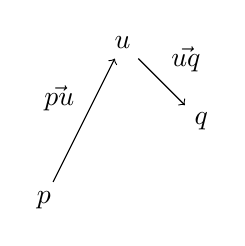
\begin{tikzpicture}
        \node (p) at (0, 0) {$p$};
        \node (u) at (1, 2) {$u$};
        \node (q) at (2, 1) {$q$};

        \graph {(p) ->["$\vec{pu}$"] (u)};
        \graph {(u) ->["$\vec{uq}$"] (q)};
    \end{tikzpicture}
    \caption{Two vectors induced by three points in the plane. The path 
             $p, u, q$ makes a right-hand turn.}
    \label{fig:orient1}
    \end{subfigure}\hfill
    \begin{subfigure}{0.45\textwidth}
    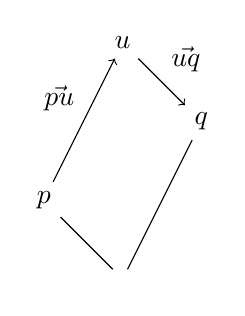
\begin{tikzpicture}
        \node (p) at (0, 0)  {$p$};
        \node (u) at (1, 2)  {$u$};
        \node (q) at (2, 1)  {$q$};
        \node (c) at (1, -1) {};

        \graph {(p) ->["$\vec{pu}$"] (u)};
        \graph {(u) ->["$\vec{uq}$"] (q)};
        \graph {(p) --               (c)};
        \graph {(c) --               (q)};
    \end{tikzpicture}
    \caption{Parallelogram spanned by $\vec{pu}$ and $\vec{uq}$. 
             The area of this parallelogram is $|orient(p, u, q)|$.}
    \label{fig:orient2}
    \end{subfigure}
    \caption{A visualisation of the orientation of three points.}
\end{figure}

We can view these as vectors in 3D by adding a $z$-coordinate $0$. Now the
cross product $\vec{pu} \times \vec{uq}$ is equal to 

\[
    \begin{pmatrix}
        0 \\
        0 \\
        (u_x - p_x) \cdot (q_y - u_y) - (u_y - p_y) \cdot (q_x - u_x)
    \end{pmatrix}.
\]

We write $orient(p, q, u)$ for the $z$-coordinate
$(q_x - p_x) \cdot (u_y - q_y) - (q_y - p_y) \cdot (u_x - q_x)$. 
If the cross-product points up, so if $orient(p, u, q) > 0$, we make a left-hand 
turn going from $p$ to $u$ to $q$, and if this is negative, we make a right-hand
turn. If it is zero, the points $p, u, q$ are collinear. 

We colloquially say $u$ is to the left of $pq$ if $orient(p, u, q) > 0$.

The authors of \cite{quickerthanqhull} point out that we can use the 
orientation to find the point furthest from the line segment $pq$. 
The norm of the outer product
$|\vec{pq} \times \vec{qu}| = |orient(p, q, u)|$ is the area of the
parallelogram spanned by $\vec{pq}$ and $\vec{qu}$. This is also equal to
the length of $pq$ multiplied by the distance from $u$ to the line through 
$pq$. So $|orient(p, u, q)| > |orient(p, u', q)|$ if and only if $u$ is further
from $pq$ than $u'$.

This cumulates into Algorithm~\ref{alg:quickhull_basic}. 

\subsection{Perfomance Considerations}

We review some factors that are relevant to performance on a Central Processing
Units (\textit{CPU}).

\subsubsection{Branching}

Whenever a CPU encounters a conditional jump \textemdash{:~generated by 
if statements and loops in high level languages~\textemdash{} it will guess 
whether to jump or not and start executing. This is also called branching.

This mechanism makes branching practically free if the correct guesses are made.
If not, the CPU must make an expensive recovery. 

\subsubsection{Vectorisation}

A \textit{vector} or \textit{SIMD} instruction is one that operates on
multiple primitive types (such as integers or floating point numbers) at
the same time. The number of elements is called the \textit{vector width},
and is typically between $2$ and $8$ elements.

Such instructions can be used to do multiple arithmetic operations such as
\texttt{a[0] = b[0] + c[0]; a[1] = b[1] + c[1];} in one instruction, but
also data-movement such as 
\texttt{a[0] = flag[0] ? b[0] : c[0]; a[1] = flag[1] ? b[1] : c[1];}.
This reduces the number of instructions necessary, and can be used to
eliminate branches.

\subsubsection{Memory Hierarchy and Multithreading}

The speed at which we can do a computation depends on how quickly we can
execute instructions, and on how quickly we can get the necessary data loaded
in registers. We call applications limited by the former \textit{compute-bound},
and applications limited by the latter \textit{memory-bound}.

Random Access Memory (\textit{RAM}) is a separate from the CPU. The bus
connecting the CPU to RAM is shared by all cores. So while using more cores
linearly increases the computational power available, it does not increase
the available bandwidth. This can turn problems that are compute-bound on
one core memory-bound when using all available cores.

Note that this only holds for a single physical CPU. It is possible to setup
systems with multiple physical CPUs that look like a single CPU from the
programmer's perspective. In that case, using cores from the different CPUs
does increase the available bandwidth.


\section{Quickhull}

\tkcomment{TODO: make the notation consistent}

The Quickhull algorithm makes use of two important facts illustrated by 
Figure~\ref{fig:quickhull}. Firstly, if $p$, $q$ are in the convex hull, then 
any point $u$ with maximum distance to the line $\vec{pq}$, is in the convex 
hull as well. Secondly, any point within the triangle $pqu$ is not in the 
convex hull. Only the points to the left of $pu$ and to the right of $uq$ 
still need to be considered.

\begin{figure}[ht]
\resizebox{\columnwidth}{!}{%
        \begin{tikzpicture}
            \node (26_32) at (5.200, 6.400) {$\bullet$};
            \node (26_9) at (5.200, 1.800) {$\bullet$};
            \node (27_49) at (5.400, 9.800) {$\bullet$};
            \node (37_18) at (7.400, 3.600) {$\bullet$};
            \node (9_18) at (1.800, 3.600) {$\bullet$};
            \node (16_14) at (3.200, 2.800) {$\bullet$};
            \node (40_13) at (8.000, 2.600) {$\bullet$};
            \node (22_17) at (4.400, 3.400) {$\bullet$};
            \node (34_2) at (6.800, 0.400) {$\bullet$};
            \node (37_4) at (7.400, 0.800) {$\bullet$};
            \node (8_13) at (1.600, 2.600) {$\bullet$};
            \node (r1) at (2.000, 0.200) {$r_1$};
            \node (38_19) at (7.600, 3.800) {$\bullet$};
            \node (r2) at (9.400, 9.200) {$r_2$};
            \node (38_25) at (7.600, 5.000) {$\bullet$};
            \node (11_16) at (2.200, 3.200) {$\bullet$};
            \node (7_38) at (1.400, 7.600) {$\bullet$};
            \node (27_37) at (5.400, 7.400) {$\bullet$};
            \node (37_14) at (7.400, 2.800) {$\bullet$};
            \node (5_48) at (1.000, 9.600) {$\bullet$};
            \node (34_21) at (6.800, 4.200) {$\bullet$};
            \node (14_24) at (2.800, 4.800) {$\bullet$};
            \node (35_36) at (7.000, 7.200) {$\bullet$};
            \node (43_21) at (8.600, 4.200) {$\bullet$};
            \node (40_30) at (8.000, 6.000) {$\bullet$};
            \node (25_48) at (5.000, 9.600) {$\bullet$};
            \node (46_37) at (9.200, 7.400) {$\bullet$};
            \node (q) at (9.800, 6.800) {$q$};
            \node (8_49) at (1.600, 9.800) {$\bullet$};
            \node (31_48) at (6.200, 9.600) {$\bullet$};
            \node (26_42) at (5.200, 8.400) {$\bullet$};
            \node (14_35) at (2.800, 7.000) {$\bullet$};
            \node (32_41) at (6.400, 8.200) {$\bullet$};
            \node (22_21) at (4.400, 4.200) {$\bullet$};
            \node (7_29) at (1.400, 5.800) {$\bullet$};
            \node (19_41) at (3.800, 8.200) {$\bullet$};
            \node (1_33) at (0.200, 6.600) {$\bullet$};
            \node (16_38) at (3.200, 7.600) {$\bullet$};
            \node (19_11) at (3.800, 2.200) {$\bullet$};
            \node (9_12) at (1.800, 2.400) {$\bullet$};
            \node (42_36) at (8.400, 7.200) {$\bullet$};
            \node (10_38) at (2.000, 7.600) {$\bullet$};
            \node (25_12) at (5.000, 2.400) {$\bullet$};
            \node (22_33) at (4.400, 6.600) {$\bullet$};
            \node (13_5) at (2.600, 1.000) {$\bullet$};
            \node (31_39) at (6.200, 7.800) {$\bullet$};
            \node (p) at (0.000, 9.400) {$p$};
            \node (24_32) at (4.800, 6.400) {$\bullet$};
            \node (40_47) at (8.000, 9.400) {$\bullet$};
            \node (6_47) at (1.200, 9.400) {$\bullet$};

            \graph {(p) --[red] (q)};
            \graph {(p) --[red] (r1)};
            \graph {(r1) --[red] (q)};
            \graph {(p) --[red] (r2)};
            \graph {(r2) --[red] (q)};
        \end{tikzpicture}
    }
    \caption{The points $p$ and $q$ are the left-most and 
             right-most points, and therefore in the hull. The points $r_1$,
             $r_2$ are furthest from the line $pq$, and also in the hull. Any
             point within the two triangles cannot be in the convex hull.}
    \label{fig:quickhull}
\end{figure}

This idea can be applied recursively to find the complex hull, starting with
the left-most (highest in case of ties), and right-most (lowest in case of ties)
points.

\subsection{Orientation}

While it is intuitively clear what points are to the left of a line $pr$, or
inside a triangle $prq$, it is not straightforward to define this precisely.
For this we need a quantity called the orientation of three points.

Given three points $p, q, u$ in the plane, we have vectors
\[
    \vec{pq} = \begin{pmatrix}
        q_x - p_x \\
        q_y - p_y
    \end{pmatrix},
    \vec{qu} = \begin{pmatrix}
        u_x - q_x \\
        u_y - q_y
    \end{pmatrix}
\]

representing oriented line segments between the points, as depicted in
Figure~\ref{fig:orient1}.

\begin{figure}[ht]
    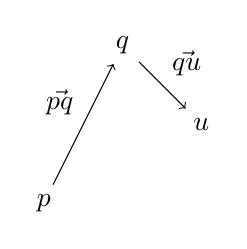
\begin{tikzpicture}
        \node (p) at (0, 0) {$p$};
        \node (q) at (1, 2) {$q$};
        \node (u) at (2, 1) {$u$};

        \graph {(p) ->["$\vec{pq}$"] (q)};
        \graph {(q) ->["$\vec{qu}$"] (u)};
    \end{tikzpicture}
    \caption{Two vectors induced by three points in the plane. The path 
             $p, q, u$ makes a right-hand turn.}
    \label{fig:orient1}
\end{figure}

We can view these as vectors in 3D by adding a $z$-coordinate $0$. Now the
cross product $\vec{pq} \times \vec{qu}$ is equal to 

\[
    \begin{pmatrix}
        0 \\
        0 \\
        (q_x - p_x) \cdot (u_y - q_y) - (q_y - p_y) \cdot (u_x - q_x)
    \end{pmatrix}.
\]

We write $orient(p, q, u)$ for the $z$-coordinate
$(q_x - p_x) \cdot (u_y - q_y) - (q_y - p_y) \cdot (u_x - q_x)$. 
If the cross-product points up, so if $orient(p, q, u) > 0$, we make a left-hand 
turn going from $p$ to $q$ to $u$, and if this is negative, we make a right-hand
turn. If it is zero, the points $p, q, u$ are colinear. 

We colloquially say $u$ is to the left of $pq$ if $orient(p, u, q) > 0$.

The authors of \cite{quickerthanqhull} point out that we can use the 
orientation to find the point furthest from the line segment $pq$. 
The norm of the outerproduct
$|\vec{pq} \times \vec{qu}| = |orient(p, q, u)|$ is the area of the
parallelogram spanned by $\vec{pq}$ and $\vec{qu}$. This is also equal to
the length of $pq$ multiplied by the distance from $u$ to the line through 
$pq$. So $|orient(p, q, u)| > |orient(p, q, u')|$ if and only if $u$ is further
from $pq$ than $u'$. 

\begin{figure}[ht]
    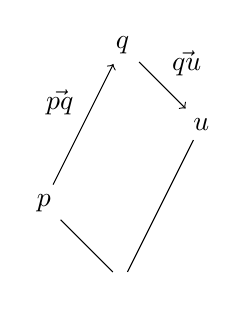
\begin{tikzpicture}
        \node (p) at (0, 0)  {$p$};
        \node (q) at (1, 2)  {$q$};
        \node (u) at (2, 1)  {$u$};
        \node (c) at (1, -1) {};

        \graph {(p) ->["$\vec{pq}$"] (q)};
        \graph {(q) ->["$\vec{qu}$"] (u)};
        \graph {(p) --               (c)};
        \graph {(c) --               (u)};
    \end{tikzpicture}
    \caption{Parallellogram spanned by $\vec{pq}$ and $\vec{qu}$. 
             The area of this parallelogram is $|orient(p, q, u)|$.}
    \label{fig:orient2}
\end{figure}

This cumulates into Algorithm~\ref{alg:quickhull_basic}. By slight abuse
of notation, we assume that the sets are ordered, so that in $\{p\} \cup \{q\}$,
the point $q$ comes after $p$.

\begin{algorithm}[ht]
\begin{algorithmic}[1]
    \caption{Quickhull algorithm}\label{alg:quickhull_basic}
    \Require $P: $ set of points in $\mathbb{R}^2$,
    \Ensure $H: $ vertices of convex hull of $P$ in clockwise order.
    \State Let $p$ be the left-most point in $P$, $q$ the right-most point.
    \State Let $S_1 = \{u \in P \ | \ orient(p, u, q) > 0\}$
    \State Let $r_1 = \argmax\limits_{u \in S_1}orient(p, u, q)$.
    \State Let $S_2 = \{u \in P \ | \ orient(q, u, p) > 0\}$
    \State Let $r_2 = \argmax\limits_{u \in S_2}orient(q, u, p)$.
    \State Let $H = \{p\} \cup $ \Call{FindHull}{$S_1$, $p$, $r_1$, $q$}
            $\cup \{q\} \cup$ \Call{FindHull}{$S_2$, $q$, $r_2$, $p$}.
    \Function{FindHull}{P, p, r, q}
        \If{$|P| \leq 1$}
            \State Let $H = P$.
        \Else
            \State Let $S_1 = \{u \in P \ | \ orient(p, u, r) > 0\}$.
            \State Let $r_1 = \argmax\limits_{u \in S_1}orient(p, u, r)$.
            \State Let $S_2 = \{u \in P \ | \ orient(r, u, q) > 0\}$
            \State Let $r_2 = \argmax\limits_{u \in S_2}orient(r, u, q)$.
            \State Let $H = \{p\} \cup $ \Call{FindHull}{$S_1$, $p$, $r_1$, $r$}
                   $\cup \{q\} \cup$ \Call{FindHull}{$S_2$, $r$, $r_2$, $q$}
        \EndIf
    \EndFunction
\end{algorithmic}
\end{algorithm}

\subsection{Accuracy}

\tkcomment{Before I forget: right now we need orient(p, p, q) = orient(p, q, q) = 0
in order for the algorithm to terminate. This forces us to evaluate the orientation
the way described. However, this leads to us finding only 10\% of the points out of
100M. That is laughable as we have 53 bits of mantissa. By finding the index of $r_i$
instead of $r_i$, we can eliminate $r_i$ before calling the recursive function,
which guarantees algorithm termination. We then have free reign into evalulating
orient accurately. There is much literature on this. Search terms: Kahan Determinant
FMA, accurate sign}

%\subsection{Performance Considerations}
%
%In order to optimize Quickhull, we focussed on the following three optimisation
%goals: minimising data movement, minimizing cache misses, and effective 
%parallelisation.
%
%\subsubsection{Data Movement}
%
%Doing computations quicker is only helpful so long as the input and output of
%these computations can be written from and to memory quickly enough. Our
%machine can compute $c = ab + c$ with one core a factor $4.625$ faster than it 
%can load $a, b, c$ from RAM and store the updated $c$ to RAM. Using more cores
%increases the number of computations we can do linearly, but they all share the
%same bandwidth to RAM. For this reason it is important to keep data that is used
%multiple times in cache.
%
%% 2 avx2 fma instructions per clock, 3.7 GHz, so 2 * 4 * 3.7 G instructions per 
%% second. Bandwidth is 204.8 GB/s, and we need 4 * 8 = 32 bytes per fma
%% 2 * 4 * 3.7 / (204.8 / 32) = 4.625
%
%The recursive structure of the algorithm ensures that eventually the subproblem 
%of \texttt{FindHull} will fit in cache.
%
%Caches always read and write contiguous blocks of memory to RAM and other caches,
%called cachelines. For our architecture, this is $64$ bytes. A single point is 
%$16$ bytes, so if a subset $S_1$ of $P$ is strung out across memory, only 
%$\frac{16}{64} = \frac{1}{4}$th of the cache contains useful data. For this 
%reason, we choose to permute $P$ so that it first contains $S_1$ and then $S_2$.
%This allows us to fully use the cache. Furthermore, the CPU will speculatively
%load memory into its caches to hide latency, and does so best on linear
%(or regularly strided) accesses. We also compute $r_1$, $r_2$ in the same pass
%to avoid data movement.
%
%PBBS choses to keep the indices instead. The higher the reuse, the more this
%will hurt performance because of the cache behaviour.
%
%\subsubsection{Branch Misses}
%
%Branching, that is jumping to a different section of the code depending on 
%whether a condition is met, is expensive. For this reason, CPUs will try to
%predict the branch and speculatively. If this prediction is wrong, this
%speculative execution has to be rolled back. This is known to be very expensive
%in the context of the algorithmically similar Quickhull \cite{}. Fortunately,
%branches can be avoided with clever programming \cite{}.
%
%Inspired by ips4o \cite{}, we first permute $P$ such that each block of $b$
%points ($64$ in our implementation) contains points that exclusively belong
%to $S_1$ or $S_2$. Unlike ips4o, we do not need to keep points that belong in
%neither $S_1$ or $S_2$, and we do not in order to save the costs of writing them
%back. The full implementation can be found in \cite{}, but the key idea is
%the code fragment in Listing~\ref{listing:tripartition}.
%
%\begin{lstlisting}[gobble=8, captionpos=b, label=listing:tripartition,
%                   caption={Branchless Local Classification.}]
%        while (i < n && count1 < block_size && count2 < block_size) {
%            double o1 = orient(p, P[i], r);
%            double o2 = orient(r, P[i], q);
%
%            buf1[count1] = P[i];
%            buf2[count2] = P[i];
%            orient1[count1] = o1;
%            orient2[count2] = o2;
%
%            count1 += (o1 > 0);
%            count2 += (o2 > 0 && !(o1 > 0));
%
%            i++;
%        }
%\end{lstlisting}
%
%Here \texttt{buf1} is a block that will contain the elements of $P$ that belong
%in $S_1$. We always write \texttt{P[i]}, but only increase the location we write
%to if it belongs in $S_1$, ensuring that points not belonging in \texttt{buf1}
%will be overwritten. This is all branchless, and we fill \texttt{buf1}, 
%\texttt{buf2} up this way. Whenever a buffer is full, we write it back to $P$.
%Due to round-off errors in floating point arithmetic, it can happen that 
%\texttt{o1 > 0} and \texttt{o2 > 0}. To avoid out-of-bound accesses, we only 
%put \texttt{P[i]} in \texttt{buf2} if it is not in \texttt{buf1}.
%
%After this phase, we reorder the blocks using a Hoare partitioning, and insert
%the points in \texttt{buf1}, \texttt{buf2} that had not been written back yet. 
%This means we pass over the data twice, while it is possible to do it in one,
%by using the Dutch Flag Algorithm, increasing the demand on the bandwidth.
%However, this method is cache-friendly as we always read and write entire 
%cachelines, and points not in $S_1$, $S_2$ are not considered for the second 
%pass. This ensures very reasonable performance in practice.
%
%\tkcomment{TODO Quantify 'very reasonable'}
%
%\subsubsection{Parallelism}
%
%We need to both parallelise the partitioning, as well as the recursive calls.
%
%\begin{figure}[h]
%    \resizebox{\columnwidth}{!}{%
%        \begin{tikzpicture}
%            \foreach \i in {0, ..., 12} {
%                \draw (\i, 0) rectangle (\i + 1, 1);
%            }
%            \foreach \i in {0, ..., 3} {
%                \node at (3 * \i + 0.5, 0.5) {$?$};
%            }
%
%            \draw[->, red, thick] (5, -0.1) -- (5, -0.9);
%            \node at (7, -0.5) {Local Classification};
%
%            \foreach \i in {0, ..., 12} {
%                \draw (\i, -2) rectangle (\i + 1, -1);
%            }
%            \foreach \i in {0, ..., 2} {
%                \node at (3 * \i + 0.5, -1.5) {$S_{?}$};
%            }
%            \foreach \i in {3} {
%                \node at (3 * \i + 0.5, -1.5) {$-$};
%            }
%
%            \draw[->, red, thick] (5, -2.1) -- (5, -2.9);
%            \node at (7, -2.5) {Hoare Permutation};
%
%            \foreach \i in {0, ..., 12} {
%                \draw (\i, -4) rectangle (\i + 1, -3);
%            }
%            \node at (0.5, -3.5) {$S_1$};
%            \node at (3.5, -3.5) {$S_1$};
%            \node at (6.5, -3.5) {$S_2$};
%            \node at (9.5, -3.5) {$-$};
%        \end{tikzpicture}
%    }
%    \caption{Parallel Partitioning by thread 0 out of 3 threads total}
%\end{figure}
%
%


\section{Performance Considerations}

\tkcomment{TODO: short explanation of the big-three: bandwidth, vectorization, branch misprediction}


\section{partitioning}

In Quicksort, we partition our input into two sets: those smaller than the 
pivot, and those larger or equal. The situation in Quickhull is more similar
to the Dutch National Flag Problem, with the following three options for each
point: belonging in $S_1$, in $S_2$, or neither. The key difference is that
we do not need to preserve the points belonging in neither. This allows us
to modify the more efficient algorithms for bipartitioning.


\subsection{Sequential Partitioning}

Bramas showed in \cite{} that it is possible to vectorize the partitioning
of Quicksort. This is done by reading a vector of values from either the
left or right of the array, partitioning this vector in registers, and
then writing it back to the front and back of the array. During this process,
the invariant of Figure~\ref{fig:invariant_bramas} is maintained.

\begin{figure}[ht]
    \resizebox{\columnwidth}{!}{%
        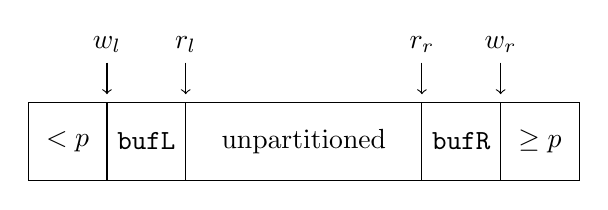
\begin{tikzpicture}
            \draw (0, 0) rectangle (1, 1) node[midway] {$< p$};
            \draw (1, 0) rectangle (2, 1) node[midway] {\texttt{bufL}};
            \draw (2, 0) rectangle (5, 1) node[midway] {unpartitioned};
            \draw (5, 0) rectangle (6, 1) node[midway] {\texttt{bufR}};
            \draw (6, 0) rectangle (7, 1) node[midway] {$\geq p$};

            \draw[->] (1, 1.5) node[above] {$w_l$} -- (1, 1.1);
            \draw[->] (2, 1.5) node[above] {$r_l$} -- (2, 1.1);
            \draw[->] (5, 1.5) node[above] {$r_r$} -- (5, 1.1);
            \draw[->] (6, 1.5) node[above] {$w_r$} -- (6, 1.1);
        \end{tikzpicture}
    }
    \caption{Invariant for partitioning an array into values smaller than
             a pivot $p$ and larger or equal than $p$. The values in
             \texttt{bufL}, \texttt{bufR} are buffered and can be safely
             overwritten. A write and a read pointer are maintained for
             the left and right side of the array.}
    \label{fig:invariant_bramas}
\end{figure}

Let $d$ be the number of element fitting in a vector register. The invariant
is started with \texttt{bufL} and \texttt{bufR} having space of at least
$d$ elements. As we read and write $d$ elements per iteration, the sum
of $r_l - w_l$ and $w_r - r_r$ stays $2d$, ensuring that at least one side
has enough space to write $d$ elements to.

There is enough space on the left whenever

\begin{multline}
(r_l - w_l) \geq d \iff r_l - w_l \geq 2d - (r_l - w_l) \\
\iff r_l - w_l \geq w_r - r_r.
\label{eq:bramas}
\end{multline}

In this case there is already enough space on the left, so we take this as
condition to read $d$ elements from the right. Analogously, there is enough
space of the right when this condition does not hold.

Though Bramas uses a specific avx512 instruction to partition the vector,
the authors of \cite{} show that this can be done in a portable manner by using
the Highway library \cite{}.

We use almost the same algorithm: we write points belonging in $S_1$ to the
left, and points in $S_2$ to the right. As we may write back less than
$d$ elements, we get some undefined parts of the array as illustrated in
Figure~\ref{fig:invariant_qhull}.

\begin{figure}[ht]
    \resizebox{\columnwidth}{!}{%
        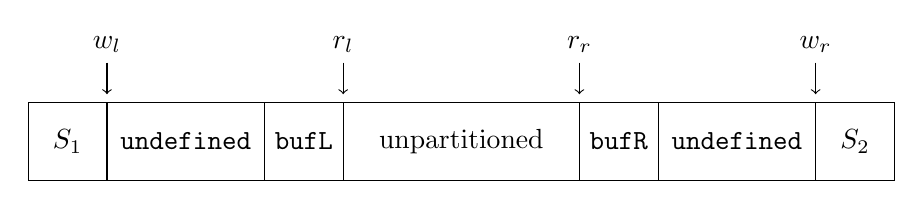
\begin{tikzpicture}
            \draw (0, 0)  rectangle (1, 1)  node[midway] {$S_1$};
            \draw (1, 0)  rectangle (3, 1)  node[midway] {\texttt{undefined}};
            \draw (3, 0)  rectangle (4, 1)  node[midway] {\texttt{bufL}};
            \draw (4, 0)  rectangle (7, 1)  node[midway] {unpartitioned};
            \draw (7, 0)  rectangle (8, 1)  node[midway] {\texttt{bufR}};
            \draw (8, 0)  rectangle (10, 1) node[midway] {\texttt{undefined}};
            \draw (10, 0) rectangle (11, 1) node[midway] {$S_2$};

            \draw[->] (1,  1.5)  node[above] {$w_l$} -- (1,  1.1);
            \draw[->] (4,  1.5)  node[above] {$r_l$} -- (4,  1.1);
            \draw[->] (7,  1.5)  node[above] {$r_r$} -- (7,  1.1);
            \draw[->] (10, 1.5)  node[above] {$w_r$} -- (10, 1.1);
        \end{tikzpicture}
    }
    \caption{Invariant for partitioning a set of points $P$ into 
             $S_1$ and $S_2$ as described in 
             Algorithm~\ref{alg:quickhull_basic}. 
             The values in \texttt{bufL}, \texttt{bufR}
             are buffered and can be safely overwritten. The values marked
             as undefined are not buffered and can be safely overwritten.
             A write and a read pointer are maintained for
             the left and right side of the array.}
    \label{fig:invariant_qhull}
\end{figure}

As $(r_l - w_l) + (w_r - r_r) \geq 2d$, the inequalities of 
Equation~\ref{eq:bramas} hold in our case as well.

\subsection{Parallel Partitioning}

Partitioning has linear complexity, so it is very likely to be limited by
bandwidth. For this reason, minimizing data-movement is the primary design goal
of the parallel algorithm. The algorithm consists out of two conceptual steps:
a parallel step where each thread works on a subset of $P$ local to it, and 
a sequential cleanup step. 

\subsubsection{Local Partition}

We first divide the points over the threads in block-cyclic fashion 
(Figure~\ref{fig:blockcycl}) according to some block parameter $b$.

\begin{figure}[ht]
    \resizebox{\columnwidth}{!}{%
        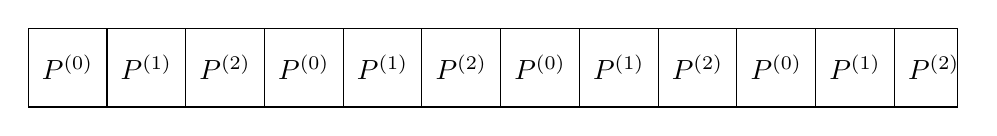
\begin{tikzpicture}
            \foreach \i in {0, ..., 10} {
                \draw (\i, 0) rectangle (\i + 1, 1);
            }
            \draw (11, 0) rectangle (11.8, 1);

            \foreach \i in {0, ..., 3} {
                \node at (3 * \i + 0.5, 0.5) {$P^{(0)}$};
            }
            \foreach \i in {0, ..., 3} {
                \node at (3 * \i + 1.5, 0.5) {$P^{(1)}$};
            }
            \foreach \i in {0, ..., 3} {
                \node at (3 * \i + 2.5, 0.5) {$P^{(2)}$};
            }
        \end{tikzpicture}
    }
    \caption{Block cyclic distribution over $3$ threads. Each square represents
             $b$ elements, except the last one that may contain less.}
    \label{fig:blockcycl}
\end{figure}

To be more precise, given $n$ points total and $n_t$ threads, we partition
the index set $I = [0, n)$ into

$$I^{(t)} = \{t \cdot b + l \cdot n_t \cdot b + j \ | \ 0 \leq j < b,
                0 \leq t \cdot b + l \cdot n_t \cdot b + j < n\}$$

for $t = 0, \cdots, n_t - 1$. Thread $t$ can then work on its subset
$P^{(t)} := \{P[i] \ | \ i \in I^{(t)}\}$ independently from the other threads.

We have each thread partition its $P^{(t)}$ in parallel, returning 
$c_{1}^{(t)}, c_{2}^{(t)} \in I^{(t)}$ such that
$\{P[i] \ | \ i \in I^{(t)}, i < c^{(t)}\} \subseteq S_1$
and $\{P[i] \ | \ i \in I^{(t)}, c^{(t)} \leq i\} \subseteq S_2$.
Denoting $c_{l}^{\min / \max}$ for the minimum / maximum of $c_1$, $c_2$, this
gives us a permuted $P$ where indices in $[0, c_1^{min})$ belong to $S_1$,
indices in $[c_{1}^{\max}, c_2^{\min})$ are in $(S_1 \cup S_2)^c$, and
indices in $[c_2^{\max}, n)$ are in $S_2$, as depicted in 
Figure~\ref{fig:local_part}.

The key observation is that for random $P$ and $n_t, b \ll n$, the ratio 
$|S_1| : |S_2|$ is roughly equal to $|S_1 \cap P^{(t)}| : |S_2 \cap P^{(t)}|$.
This means that the $c_1^{(t)}$s are expected to be close to each other, and
the global $c_1$, and likewise for the $c_2^{(t)}$s. This even holds for $P$
not random, but already a convex hull listed in clockwise, or counter-clockwise
order. So permuting $[c_1^{min}, c_1^{\max}) \cup [c_2^{min}, c_2^{\max})$
is not performance critical.

\begin{figure}[ht]
    \resizebox{\columnwidth}{!}{%
        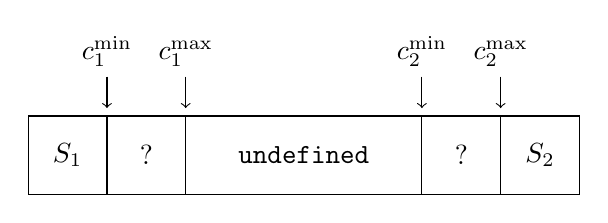
\begin{tikzpicture}
            \draw (0, 0) rectangle (1, 1) node[midway] {$S_1$};
            \draw (1, 0) rectangle (2, 1) node[midway] {$?$};
            \draw (2, 0) rectangle (5, 1) node[midway] {$\texttt{undefined}$};
            \draw (5, 0) rectangle (6, 1) node[midway] {$?$};
            \draw (6, 0) rectangle (7, 1) node[midway] {$S_2$};

            \draw[->] (1, 1.5) node[above] {$c_1^{\min}$} -- (1, 1.1);
            \draw[->] (2, 1.5) node[above] {$c_1^{\max}$} -- (2, 1.1);
            \draw[->] (5, 1.5) node[above] {$c_2^{\min}$} -- (5, 1.1);
            \draw[->] (6, 1.5) node[above] {$c_2^{\max}$} -- (6, 1.1);
        \end{tikzpicture}
    }
    \caption{The points $P$ after local partition. The points in $?$ can
             belong to either $S_1$, $S_2$, or can be undefined.}
    \label{fig:local_part}
\end{figure}

\subsubsection{Cleanup}

\tkcomment{Not yet implemented.}

In essence, the cleanup step is a Dutch National Flag Problem \cite{}: 
we have to partition into $S_1$, undefined points, $S_2$. If a point has not 
been moved, we can classify it by determining which $P^{(t)}$ its index belongs 
to, and then compare it against $c_1^{(t)}, c_2^{(t)}$. Unfortunately, the
standard algorithm proposed by Dijkstra moves some points twice, so we have
to make some modifications.

To simplify the analysis, we pretend the set we are working on is indexed
$[0, m)$.

We maintain three pointers $i \leq j < k$ and the following invariant: 
$P[0, i) \subseteq S_1$, $[i, j) \subseteq S_2$, $P[j, k)$ still have to be
sorted, $P[k, m)$ are undefined (Figure~\ref{fig:dnf}). As we can only 
classify points by comparing their index to $c_1^{(t)}, c_2^{(t)}$, we 
additionally require that inspected points have not been moved in a previous
iteration.

\begin{figure}[ht]
    \resizebox{\columnwidth}{!}{%
        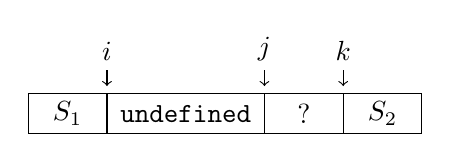
\begin{tikzpicture}
            \draw (0, 0) rectangle (1, 0.5) node[midway] {$S_1$};
            \draw (1, 0) rectangle (3, 0.5) node[midway] {$\texttt{undefined}$};
            \draw (3, 0) rectangle (4, 0.5) node[midway] {$?$};
            \draw (4, 0) rectangle (5, 0.5) node[midway] {$S_2$};

            \draw[->] (1, 0.8) node[above] {$i$} -- (1, 0.6);
            \draw[->] (3, 0.8) node[above] {$j$} -- (3, 0.6);
            \draw[->] (4, 0.8) node[above] {$k$} -- (4, 0.6);
        \end{tikzpicture}
    }
    \caption{The invariant for our Dutch National Flag variant.}
    \label{fig:dnf}
\end{figure}

\begin{algorithm}[ht]
\begin{algorithmic}[1]
    \caption{Dutch National Flag}\label{alg:dnf}
    \Require Points $P$, considered on indices $[start, end)$.
    \Ensure Permuted $P[start, end)$ and $i, j$, such that
            $P[start, i) = P[start, end) \cap S_1$ and
            $P[k, j) = P[start, end) \cap S_2$.
    \State Let $i = j = start$, $k = end$.
    \While{$j < k$}
        \If{$P[j] \in S_1$}
            \State $P[i] = P[j]$
            \State $i = i + 1$
            \State $j = j + 1$
        \ElsIf{$P[j] \notin S_1 \cup S_2$}
            \State $j = j + 1$
        \Else
            \State $k = k - 1$
            \While{$P[k] \in S_2$}
                \State $k = k - 1$
                \If{$k = j$}
                    \State \Return{}
                \EndIf
            \EndWhile
            \If{$P[k] \in S_1$}
                \State $P[i] = P[k]$
                \State $i = i + 1$
            \EndIf
            \State $P[k] = P[j]$
            \State $j = j + 1$
        \EndIf
    \EndWhile
\end{algorithmic}
\end{algorithm}

\begin{proof}
    The top-level loop will eventually terminate with $P[j, k)$ empty as 
    $j$ is incremented every iteration. 

    It is clear that the invariant is respected in the cases $P[j] \in S_1$
    and $P[j] \notin S_1 \cup S_2$.
\end{proof}

If $c_1^{\max} \leq c_2^{\min}$, we employ Algorithm~\ref{alg:dnf} with
$start = [c_1^{\min}$, $end = c_2^{\max})$, giving us 
(Figure~\ref{fig:dnf_cleanup1}). Moving $[i, j)$ up is then straightforward.

\begin{figure}[ht]
    \resizebox{\columnwidth}{!}{%
        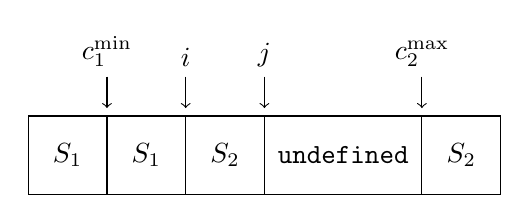
\begin{tikzpicture}
            \draw (0, 0) rectangle (1, 1) node[midway] {$S_1$};
            \draw (1, 0) rectangle (2, 1) node[midway] {$S_1$};
            \draw (2, 0) rectangle (3, 1) node[midway] {$S_2$};
            \draw (3, 0) rectangle (5, 1) node[midway] {\texttt{undefined}};
            \draw (5, 0) rectangle (6, 1) node[midway] {$S_2$};

            \draw[->] (1, 1.5) node[above] {$c_1^{\min}$} -- (1, 1.1);
            \draw[->] (2, 1.5) node[above] {$i$} -- (2, 1.1);
            \draw[->] (3, 1.5) node[above] {$j$} -- (3, 1.1);
            \draw[->] (5, 1.5) node[above] {$c_2^{\max}$} -- (5, 1.1);
        \end{tikzpicture}
    }
    \caption{The points $P$ after local partition and Dutch National Flag
             on $[c_1^{\min}, c_2^{\max})$. We then move $[i, j)$ to
             $[c_2^{\max} - (j - i), c_2^{\max})$.}
    \label{fig:dnf_cleanup1}
\end{figure}

If $c_1^{\max} > c_2^{\min}$, we employ Algorithm~\ref{alg:dnf} twice: once
on $[c_1^{\min}, c_1^{\max})$, and once on $[c_2^{\min}, c_2^{\max})$
(Figure~\ref{fig:dnf_cleanup2}). We then, ...

\begin{figure}[ht]
    \resizebox{\columnwidth}{!}{%
        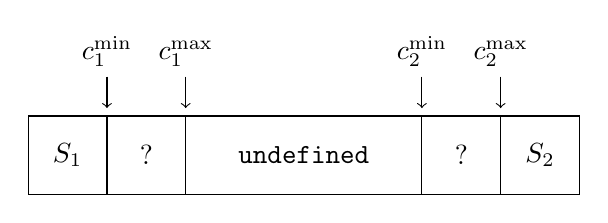
\begin{tikzpicture}
            \draw (0, 0) rectangle (1, 1) node[midway] {$S_1$};
            \draw (1, 0) rectangle (2, 1) node[midway] {$?$};
            \draw (2, 0) rectangle (5, 1) node[midway] {$\texttt{undefined}$};
            \draw (5, 0) rectangle (6, 1) node[midway] {$?$};
            \draw (6, 0) rectangle (7, 1) node[midway] {$S_2$};

            \draw[->] (1, 1.5) node[above] {$c_1^{\min}$} -- (1, 1.1);
            \draw[->] (2, 1.5) node[above] {$c_1^{\max}$} -- (2, 1.1);
            \draw[->] (5, 1.5) node[above] {$c_2^{\min}$} -- (5, 1.1);
            \draw[->] (6, 1.5) node[above] {$c_2^{\max}$} -- (6, 1.1);
        \end{tikzpicture}
    }
    \caption{The points $P$ after local partition and Dutch National Flag
             on $[c_1^{\min}, c_2^{\max})$. We then move $[i, j)$ to
             $[c_2^{\max} - (j - i), c_2^{\max})$.
             $k$ cannot be undefined, and the point under $j$ has not been 
             moved.}
    \label{fig:dnf_cleanup2}
\end{figure}

\subsubsection{Implementation Details}

\tkcomment{round down n so the reads do not cross blocks, explain how we handle
the write crossing blocks, cheap branches, false sharing, keep the index in
two integers to allow for fast checking, check whether 
$c_1^{\max} > c_2^{\min}$ etc.}


\section{Implementation}

Parallelise both the recursion and the partitioning.
Divide processors over subsets in ratio, switch to sequential when $n_t \leq 1$.
memmove to keep it in-place.

In order to minimise bandwidth use, we also weave in the compution 
of $r_1$ and $r_2$ during the partition.

\iffalse
\subsection{Optimisation considerations}

\tkcomment{Computational density is very low, so need to care about bandwidth 
(scales poorly with multiple cores), and branch misprediction (scales well).}

\subsection{Quickhull}

PBBS stores sets of points by a large array $P$ of all points, and an index 
array $I$. So the actual $P$ being considered is $\{P[i] \ | \ i \in I\}$.

In order to find $S_1$, $S_2$, Hoare's partition scheme is used on $I$, where
$i$ is considered to be than the pivot if $P[i]$ is above $pr_k$, smaller than
the pivot if $P[i]$ is below $r_kq$, and equal to the pivot if it is in the
triangle $pr_kq$. This is a fine approach for datasets where almost all points
are eliminated in the first few sweeps. When this is not the case however,
it makes inefficient use of the bandwidth. The subsets of points are scattered
throughout memory, which hurts the cache utilisation. Hoare's partitioning
method is also susceptible to branch misses. On some datasets these were as
large as $6\%$.

Instead, we decided to not use indices, but to swap the points of $P$. This 
ensures that $S_1$, $S_2$ are in contiguous memory, making 

\tkcomment{It does not make any sense PBBS is faster. It traverses the entire array to find $r$, instead of passing it into the next iteration like we do, which is inefficient. It also partitions the entire array twice, while we know that points to the left of $pr$ are also the the left of $rq$. And it does not use block partitioning. It uses and extra index array instead of checking at the same time. Maybe the swap is more expensive for points than indices?}

\subsubsection{Optimising Quickhull}

Optimisation goals: optimising branch misses and bandwidth utilisation.

We need to use a branchless partition. A branchless tri-partitioning does not 
exist to the best of my knowledge.

As for the first pass there are always little elements 'equal' to the degenerate
triangle, we could do a >= and <=, keep track of the p and q indices, and cut
those out. For Kuzmin, that would save one pass over the data. The elements on
the line not equal to $p$ or $q$ are deleted next pass anyway. That would shave
off 20 ms.
\fi


\section{Performance Evaluation}\label{sec:perf}

The PBBS benchmark consists of three data sets. Each of these consists of
$10^8$ points drawn from different distributions. Even though all data sets
are $1.6$ GB in size, the algorithm behaves very differently on them.

As a baseline we have considered Qhull, the algorithms of CGAL,
and the implementation of PBBS. Some preliminary testing shows that the
implementation of PBBS is the fastest by a large margin. In
Table~\ref{table:reference} are the runtimes for a disk of $10^7$ points.

\begin{table}[ht]
    \caption{Runtime in seconds for a disk of $10^7$ points}
    \label{table:reference}
    \begin{tabular}{c | c }
     Implementation & Runtime \\ 
     \hline \\
     PBBS & 0.31 \\  
     CGAL Quickhull & 0.61 \\
     CGAL Akl-Toussaint & 0.60 \\
     CGAL Bykat & 0.73 \\
     CGAL Eddy & 0.98 \\
     CGAL Graham & 1.3 \\
     CGAL Jarvis & 208 \\
     Qhull & TODO, but slow \\
    \end{tabular}
\end{table}

We use GCC 14.1.1. All experiments are run 20 times. The standard deviation is 
less than $2.5\%$ in all cases, so we only report the means.

\subsection{Evaluation Platforms}

We evaluate our implementation on two machines. The first, \textit{cn125}
has powerful vector instructions, a modest amount of cores and memory, and a 
simple memory architecture. 

The second, \textit{cn132}, has less powerful vector instructions and needs
to emulate the compress of ... It has two CPUs which gives it more cores
and memory bandwidth. Memory is local to one of the two CPUs, so we need
to make sure allocations are equally distributed between the two. We have
done this by running the programs under \texttt{numactl --interleaved all}.

We summarize the systems in Table~\ref{tab:system}. There can be a significant
gap between the bandwidth the RAM is capable off, and what is achievable in
practice. The STREAM benchmark \cite{} is a collection of simple functions
that can be used to measure what bandwidths can be achieved in practice.

\begin{table}
    \caption{Theoretical and practical capabilities of test systems. All four
             STREAM benchmarks obtained the same bandwidth.}
    \label{tab:system}
    \begin{tabular}{c|c|c}
                                   & cn132 & cn125          \\
        \hline                                              
        CPU                        & Epyc 7313 $(\times 2)$ 
                                           & Xeon E-2378    \\
        Vector extension           & avx2  & avx512         \\
        Frequency (GHz)            & 3.7   & 2.6            \\
        Peak compute rate (Gflops) & 1894  & 346            \\
        Theoretic bandwidth (GB/s) & 204.8 & 51.2           \\ 
        STREAM (GB/s)              & 140   & 38             \\ 
    \end{tabular}
\end{table}

\subsection{The Data Sets}\label{subsec:datasets}

There is a large difference between runtime of Quickhull on the different 
datasets.
To gain insight, we make a rough estimation of the amount of work required.
\tkcomment{I suppose we can measure this, but the work per pass over the
data may also be interesting.}

\subsubsection{Kuzmin}

Whereas Circle and Disk are symmetric, Kuzmin is very much the opposite
as illustrated in Figure~\ref{fig:kuzmin}.
The first two partitions end up with almost all points either in $S_1$ or
in $S_2$, and on the subsequent partition almost all points are discarded.
The convex hull has only $4$ points.

\begin{figure}[ht]
    \includegraphics[width=\columnwidth]{figures/rust-kuzmin.png}
    \caption{The Kuzmin dataset of $10^8$ points. The first partition only
             moves $r_1$. The second partition eliminates all remaining points.}
    \label{fig:kuzmin}
\end{figure}

\subsubsection{Circle}

A circle is convex, so all points are on the hull. As a circle is symmetric,
each recursive call of FindHull will identify an element on the hull, and
then recurse on two subsets $S_1$ and $S_2$ differing at most one in size.
That means we have $2^d$ calls at recursion depth $d$ until we hit the point 
where either $|S_1| = 1$ and $|S_2| = 0$ or vice-versa. 
As each recursive call eliminates one point, there are
$10^8 - \sum_{i = 0}^{d - 1} 2^i = 10^8 - 2^{d}$ points left at recursion 
depth $d$. For $10^8$ points, we have a recursion depth of 
$\lceil \log_{2}(10^8) \rceil = 26$.

\textbf{A note on accuracy: }as the circle has effectively area $0$, the 
points are much closer together than in the other data sets.
This causes some accuracy difficulties. Already for 100K points, 
both BlockQuickhull and PBBS do not report all points as being in the hull. Both 
implementations find the same points up to 10M points, after which they disagree
on $20$ points. These are points $u$ for which $\text{orient}(p, u, r_1) > 0$
and $\text{orient}(r_2, u, q) > 0$, so this is because of our choice to put
these in $S_1$. 

\subsubsection{Disk}

The first recursion will identify $p$, $r_1$, $q$, $r_2$ as lying on the
convex hull, and partition the points into those above and below $pq$.
Then the second partition will eliminate region V of 
Figure~\ref{fig:disk_level2}. This square has area $2$, so it will eliminate
most points: a fraction $\frac{2}{\pi} \approx 0.637$.

\begin{figure}[ht]
    \resizebox{\columnwidth}{!}{%
        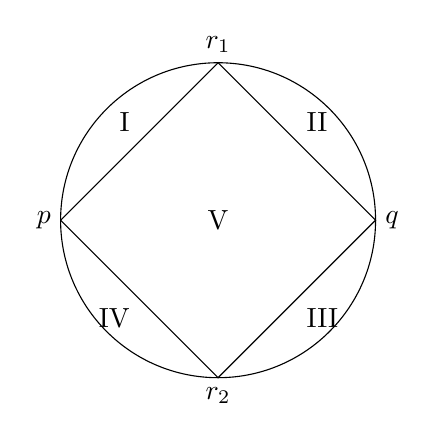
\begin{tikzpicture}
            \draw (0, 0) circle (2);
            \draw (-2, 0) node[left]  {$p$}   -- node[pos=0.5, above left] {I}
                  (0, 2)  node[above] {$r_1$} -- node[pos=0.5, above right] {II}
                  (2, 0)  node[right] {$q$}   -- node[pos=0.5, below right] {III}
                  (0, -2) node[below] {$r_2$} -- node[pos=0.5, below left] {IV}
                  (-2, 0);
                  \node at (0, 0) {V};
        \end{tikzpicture}
    }
    \caption{The Disk data set at recursion level 2. Region V will be 
             eliminated, and the recursion will continue on regions I 
             \textemdash IV.}
    \label{fig:disk_level2}
\end{figure}

After this, the recursion will continue on pie slices of progressively smaller
angle. The proportion of points eliminated is almost constant in this angle.
To see this, we label some points in Figure~\ref{fig:disk_level3+}. 

\begin{figure}[ht]
    \resizebox{\columnwidth}{!}{%
        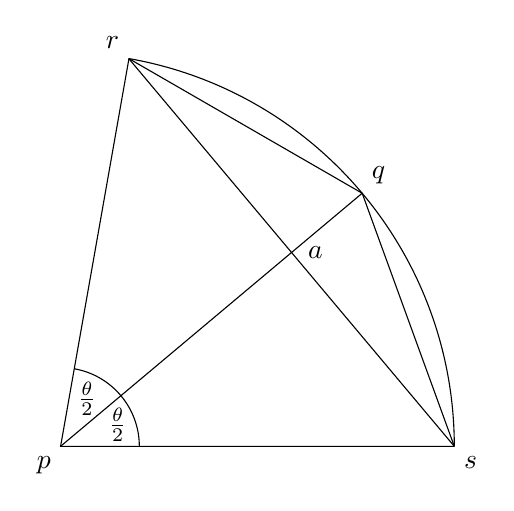
\begin{tikzpicture}
            \foreach \r in {5} {
            \draw (0,0) arc (0:80:\r);
            \draw (-0.8 * \r,0) arc (0:80:0.2 * \r) 
                            node[pos=0.2, left] {$\frac{\theta}{2}$}
                            node[pos=0.88, below] {$\frac{\theta}{2}$};
            \draw (0,0)  node[below right] {$s$} -- ++(0+180:\r) -- 
                                +(80:\r) node[above left] {$r$};
            \draw (-1 * \r,0) node[below left] {$p$} -- 
                  (0.766 * \r - 1 * \r, 0.6428 * \r) node[above right] {$q$};
            \draw (0.173 * \r - 1 * \r, 0.985 * \r) -- (0, 0);
            \draw (0.173 * \r - 1 * \r, 0.985 * \r) -- 
                  (0.766 * \r - 1 * \r, 0.6428 * \r) -- (0, 0);
            \node at (0.413 * \r - 0.766 * \r, 0.766 * 0.6428 * \r) {$a$};
        }
        \end{tikzpicture}
    }
    \caption{Subset of Disk we apply a recursive call of the Quickhull 
             algorithm on. The points are uniformly sampled from the disk
             segment to the right of the line segment $rs$.}
    \label{fig:disk_level3+}
\end{figure}

The elements not yet eliminated lie to the right of $rs$, and in this step,
we eliminate the elements in $\Delta rqs$.

The triangle $\Delta prs$ is isosceles, so $\angle par$ and $\angle pas$
are right angles. That gives us $|pa| = \cos(\theta / 2)$ and 
$|sa| = |ar| = \sin(\theta / 2)$. So $\Delta psr$ has area 
$\sin(\theta / 2) \cos(\theta / 2) = \frac{1}{2} \sin(\theta)$. The entire
pie slice has area $\frac{\theta}{2 \pi} \cdot \pi = \frac{1}{2} \theta$.
Therefore, the part of the circle above the line $rs$ has area 
$\frac{1}{2}(\theta - \sin(\theta))$.

Since $|aq| = |pq| - |pa| = 1 - \cos(\theta / 2)$, the area of $\Delta rqs$
is $\sin(\theta / 2) (1 - \cos(\theta / 2))$. So the fraction of points we
eliminate is

$$\frac{2\sin(\theta / 2) (1 - \cos(\theta / 2))}{\theta - \sin(\theta)}.$$

We approximate this with a third degree Chebyshev approximation on 
$[0, \frac{\pi}{2}]$, which is

% 1.48202191816423201 * 0.5 - -0.00314946736514754 = 0.744160426447263545
% -0.01207255984434141 - 3 * -0.00007573579005338  = -0.01184535247418127
% 2 * -0.00314946736514754                         = -0.00629893473029508
% 4 * -0.00007573579005338                         = -0.00030294316021352
$$0.744 - 0.012 \theta - 0.0063 \theta^2 - 0.0003 \theta^3. $$

The smaller $\theta$ gets, the closer this will be to $0.744$. Even for the
largest $\theta = \frac{\pi}{2}$, this value is reasonably close: $0.708$. 
So we take $0.74$ as approximation. That means the recursion depth is roughly
$1 + \log_{\frac{1}{1 - 0.74}}((1 - 0.637) \cdot 10^8) \approx 14$.

The convex hull has $1593$ points.

\subsection{Interpreting the Results}

Evaluating the performance of an algorithm and its implementation is difficult.
The runtime alone tells us little about the quality of the implementation, as
it differs between machines. We give a few performance measures that can
be related to the capabilities of the machine.

\subsubsection{Bandwidth}

To measure how good our implementation of Quickhull is, we compute the data 
movement required by Quickhull divided by the runtime. The distance between
this and the peak bandwidth of the machine, gives us an
idea of how far the implementation can be improved.

For all datasets, we need to read $10^8$ elements to find the left-most
and right-most point, and then $10^8$ reads and writes to partition $P$
in the set of points above and below the resulting line-segment. A point
is $16$ bytes, so this amounts to $16 \cdot 10^8 \cdot 3 = 4.8 GB$ of 
data-movement. After that, it depends on the data set. We can compute this 
straightforwardly from the analysis of Subsection~\ref{subsec:datasets}.


\textbf{Kuzmin:} after the initial partition into above and below $pq$ of
Figure~\ref{fig:kuzmin}, we only need one read pass to eliminate the
points in $\Delta pr_2q$. This cumulates in a data movement of

$$4.8 \cdot 10^9 + 16 \cdot 10^8 = 6.4 GB.$$ 

\textbf{Circle:} each pass reads and writes all elements in that recursion
level, so the total data movement is

$$4.8 \cdot 10^9 + 2 \cdot 16 \sum_{d = 2}^{26}(10^8 - 2^d) = 81 GB.$$


\textbf{Disk:} on the first recursion we read all points, and write
$1 - \frac{2}{\pi} \approx 0.363$ of those back. From recursion level 2 onwards,
we read all points that are left, and write only a fraction $0.26$ of those
back, so the total data movement is

$$4.8 \cdot 10^9 + (1 + 0.363) \cdot 16 \cdot 10^8 + $$
$$16 \cdot \sum_{d = 1}^{13} 
\left(0.363 \cdot 10^8 \cdot (0.26^{d - 1} + 0.26^{d})\right) =$$
$$8.0 GB.$$

\subsubsection{Effective Bandwidth}

The data movement in this algorithm is not optimal. Take for example 
Figure~\ref{fig:disk_level2}. We could have identified $p$, $r_1$, $q$, $r_2$
in one pass by also keeping track of top and bottom elements. That means
that to reach that stage, we need two reads on $10^8$ elements,
and a write on 
$\left(1 - \frac{2}{\pi}\right) \cdot 10^8 \approx 3.6 \cdot 10^7$ elements.
That would bring the total data movement down from $9.2$ GB to $5.0$ GB.

So to also take possible algorithmic improvements into account,
we also compute the bandwidth as if we did the theoretical minimum of
data movement: one read of the input, and one write for the output.

\subsubsection{Compute Rate}

Computing the orientation of a point takes $7$ flops, and this function is
evaluated twice every time an element is partitioned. So the total number of
flops required is

$$2 \cdot 7 \cdot 2 \cdot 10^8 = 2.8 \cdot 10^9,$$ 
$$2 \cdot 7 \cdot \sum_{d = 1}^{26} (10^8 - 2^d) = 34 \cdot 10^9,$$
$$2 \cdot 7 \cdot 10^8 \cdot 2 + 7 \sum_{d = 1}^{13} \left(0.363^d \cdot 
10^8 \right)  = 3.6 \cdot 10^9.$$

Every clock cycle, the vector units can do $8$ subtractions, multiplications, 
or fmas. We have these in a $4:1:1$ ratio, and they do $1, 1, 2$
flops. The frequency is $2.6$ GHz, so for our computation the peak performance
per core is

$$2.6 \cdot 8 \cdot \frac{4 \cdot 1 + 1 \cdot 1 + 1 \cdot 2}{4 + 1 + 1} = 24.3 
        \ \text{Gflops}.$$

For the entire CPU, this becomes $194$ Gflops.

\subsection{Analysis}

In contrast to our approach, PBBS does not permute the points, but instead
an array of indices pointing to the subsets. This can make for poor spatial
locality in the access of $P$, especially in deeper recursion levels.
It also inhibits vectorization.

For the Kuzmin, almost all points belong in either $S_1$ or $S_2$, so
this dataset is the exception. Similarly, the branches are easy to predict,
giving BlockQuickhull little advantage over the approach of
PBBS. For this reason, we see in Table~\ref{table:runtime} that the deeper
the recursion, the larger our lead over PBBS becomes. The only reason that
BlockQuickhull is faster on Kuzmin because Clang is able to do some 
vectorization in the partition.

Kuzmin has to get its data from RAM in all its passes, so we can expect
no more than $38$ GB/s of bandwidth. We see in Table~\ref{table:bw} that
we get $90\%$ of this. The Hoare Partition does no swaps because the
partitions are so uneven. This is not the case for Disk and Circle. However, 
they do have the advantage of a deep, symmetric recursion. This ensures
that subproblems will eventually fit in cache, which has a higher bandwidth
than RAM. As Circle has a deeper recursion and eliminates less elements,
it gets a higher bandwidth than Disk, but Table~\ref{table:ef_bw} shows it
gets a lower effective bandwidth.

The single-threaded benchmarks are not bound by memory bandwidth, yet we
see in Table~\ref{table:flops} that we achieve only a fraction of the
peak compute rate. This is partially caused by work that is not counted
towards the flop count, such as finding the left-most and right-most point,
and finding $r_1$, $r_2$. Another reason is that Clang is not able to use
SIMD instructions to their fullest potential. It vectorizes over \texttt{xmm} 
registers, which can only do two double precision elements at a time, whereas 
the available \texttt{zmm} registers can do eight. Auto-vectorization is a hard 
problem, GCC (version 14.1.1) is not able to do it at all.

% Generated with scripts

\pgfplotstableread{
Imp,Kuzmin,kuzminstd,Circle,circlestd,Disk,diskstd
PBBS,9.80e-01, 1.38e-03, 6.11e+01, 1.72e-01, 3.86e+00, 1.07e-02
VecQuickhull,2.93e-01, 1.23e-03, 4.73e+00, 1.19e-02, 4.48e-01, 1.96e-03
PBBS par,2.34e-01, 2.74e-03, 8.71e+00, 5.85e-02, 5.29e-01, 9.97e-03
VecQuickhull par,1.52e-01, 2.54e-03, 1.21e+00, 3.34e-02, 2.48e-01, 4.25e-03
}\runtimetable

\pgfplotstableread{
Imp,Kuzmin,kuzminstd,Circle,circlestd,Disk,diskstd
PBBS,6.88e-01, 3.89e-03, 5.43e+01, 1.13e-01, 3.59e+00, 1.75e-02
VecQuickhull,4.39e-01, 3.45e-03, 6.57e+00, 1.54e-02, 6.74e-01, 4.47e-03
PBBS par,7.40e-02, 4.24e-04, 3.24e+00, 1.91e-02, 1.90e-01, 3.41e-03
VecQuickhull par,5.72e-02, 2.56e-03, 3.78e-01, 2.60e-02, 9.02e-02, 1.59e-02
}\runtimetablenuma

\pgfplotstableread{
Imp,Kuzmin,kuzminstd,Circle,circlestd,Disk,diskstd
PBBS,5.71e+00, 4.04e+03, 1.19e+00, 4.23e+02, 1.86e+00, 6.73e+02
VecQuickhull,1.91e+01, 4.54e+03, 1.54e+01, 6.15e+03, 1.61e+01, 3.67e+03
PBBS par,2.39e+01, 2.05e+03, 8.38e+00, 1.25e+03, 1.36e+01, 7.22e+02
VecQuickhull par,3.70e+01, 2.20e+03, 6.05e+01, 2.19e+03, 2.90e+01, 1.69e+03
}\bwtable

\pgfplotstableread{
Imp,Kuzmin,kuzminstd,Circle,circlestd,Disk,diskstd
PBBS,8.13e+00, 1.44e+03, 1.35e+00, 6.46e+02, 2.00e+00, 4.10e+02
VecQuickhull,1.27e+01, 1.62e+03, 1.11e+01, 4.73e+03, 1.07e+01, 1.61e+03
PBBS par,7.57e+01, 1.32e+04, 2.26e+01, 3.82e+03, 3.79e+01, 2.11e+03
VecQuickhull par,9.79e+01, 2.19e+03, 1.93e+02, 2.81e+03, 7.98e+01, 4.53e+02
}\bwtablenuma

\pgfplotstableread{
Imp,Kuzmin,kuzminstd,Circle,circlestd,Disk,diskstd
PBBS,1.63e+00, 1.16e+03, 2.64e-02, 9.35e+00, 4.14e-01, 1.50e+02
VecQuickhull,5.46e+00, 1.30e+03, 3.41e-01, 1.36e+02, 3.58e+00, 8.16e+02
PBBS par,6.84e+00, 5.85e+02, 1.85e-01, 2.75e+01, 3.02e+00, 1.60e+02
VecQuickhull par,1.06e+01, 6.29e+02, 1.33e+00, 4.83e+01, 6.44e+00, 3.76e+02
}\efbwtable

\pgfplotstableread{
Imp,Kuzmin,kuzminstd,Circle,circlestd,Disk,diskstd
PBBS,2.32e+00, 4.12e+02, 2.97e-02, 1.43e+01, 4.45e-01, 9.12e+01
VecQuickhull,3.64e+00, 4.64e+02, 2.45e-01, 1.04e+02, 2.38e+00, 3.58e+02
PBBS par,2.16e+01, 3.77e+03, 4.98e-01, 8.43e+01, 8.41e+00, 4.70e+02
VecQuickhull par,2.80e+01, 6.25e+02, 4.26e+00, 6.19e+01, 1.77e+01, 1.01e+02
}\efbwtablenuma

\pgfplotstableread{
Imp,Kuzmin,kuzminstd,Circle,circlestd,Disk,diskstd
PBBS,2.86e+00, 2.02e+03, 5.56e-01, 1.97e+02, 9.32e-01, 3.36e+02
VecQuickhull,9.56e+00, 2.27e+03, 7.19e+00, 2.86e+03, 8.04e+00, 1.84e+03
PBBS par,1.20e+01, 1.02e+03, 3.90e+00, 5.81e+02, 6.81e+00, 3.61e+02
VecQuickhull par,1.85e+01, 1.10e+03, 2.82e+01, 1.02e+03, 1.45e+01, 8.47e+02
}\floptable

\pgfplotstableread{
Imp,Kuzmin,kuzminstd,Circle,circlestd,Disk,diskstd
PBBS,4.07e+00, 7.20e+02, 6.27e-01, 3.01e+02, 1.00e+00, 2.05e+02
VecQuickhull,6.37e+00, 8.12e+02, 5.17e+00, 2.20e+03, 5.34e+00, 8.05e+02
PBBS par,3.79e+01, 6.60e+03, 1.05e+01, 1.78e+03, 1.89e+01, 1.06e+03
VecQuickhull par,4.89e+01, 1.09e+03, 8.99e+01, 1.31e+03, 3.99e+01, 2.27e+02
}\floptablenuma

\tkcomment{For some reason it is really hard to get significant figures
in Latex. Maybe write a C program that generates Latex code.}

\begin{table}[ht]
    \caption{BlockQuickhull and PBBS Quickhull runtime in seconds on cn125.}
    \label{table:runtime}
    \pgfplotstabletypeset[
        columns={Imp,Kuzmin,Circle,Disk},
        column type/.add={|}{},
        every last column/.style={column type/.add={}{|}},
        every head row/.style={before row=\hline, after row=\hline},
        every last row/.style={after row=\hline},
        columns/Imp/.style={string type, column name={}},
    ]\runtimetable
\end{table}

\begin{table}[ht]
    \caption{BlockQuickhull and PBBS Quickhull runtime in seconds on cn132.}
    \label{table:runtimenuma}
    \pgfplotstabletypeset[
        columns={Imp,Kuzmin,Circle,Disk},
        column type/.add={|}{},
        every last column/.style={column type/.add={}{|}},
        every head row/.style={before row=\hline, after row=\hline},
        every last row/.style={after row=\hline},
        columns/Imp/.style={string type, column name={}},
    ]\runtimetablenuma
\end{table}

\begin{table}[ht]
    \caption{BlockQuickhull and PBBS Quickhull bandwidth in GB/s on cn125.}
    \label{table:bw}
    \pgfplotstabletypeset[
        columns={Imp,Kuzmin,Circle,Disk},
        column type/.add={|}{},
        every last column/.style={column type/.add={}{|}},
        every head row/.style={before row=\hline, after row=\hline},
        every last row/.style={after row=\hline},
        columns/Imp/.style={string type, column name={}},
    ]\bwtable
\end{table}

\begin{table}[ht]
    \caption{BlockQuickhull and PBBS Quickhull bandwidth in GB/s on cn132.}
    \label{table:bwnuma}
    \pgfplotstabletypeset[
        columns={Imp,Kuzmin,Circle,Disk},
        column type/.add={|}{},
        every last column/.style={column type/.add={}{|}},
        every head row/.style={before row=\hline, after row=\hline},
        every last row/.style={after row=\hline},
        columns/Imp/.style={string type, column name={}},
    ]\bwtablenuma
\end{table}


\begin{table}[ht]
    \caption{BlockQuickhull and PBBS Quickhull effective bandwidth in GB/s
             on cn125.}
    \label{table:ef_bw}
    \pgfplotstabletypeset[
        columns={Imp,Kuzmin,Circle,Disk},
        column type/.add={|}{},
        every last column/.style={column type/.add={}{|}},
        every head row/.style={before row=\hline, after row=\hline},
        every last row/.style={after row=\hline},
        columns/Imp/.style={string type, column name={}},
        columns/Kuzmin/.style={fixed},
        columns/Circle/.style={fixed},
        columns/Disk/.style={fixed},
    ]\efbwtable
\end{table}

\begin{table}[ht]
    \caption{BlockQuickhull and PBBS Quickhull effective bandwidth in GB/s
             on cn132.}
    \label{table:ef_bwnuma}
    \pgfplotstabletypeset[
        columns={Imp,Kuzmin,Circle,Disk},
        column type/.add={|}{},
        every last column/.style={column type/.add={}{|}},
        every head row/.style={before row=\hline, after row=\hline},
        every last row/.style={after row=\hline},
        columns/Imp/.style={string type, column name={}},
        columns/Kuzmin/.style={fixed},
        columns/Circle/.style={fixed},
        columns/Disk/.style={fixed},
    ]\efbwtablenuma
\end{table}

\begin{table}[ht]
    \caption{BlockQuickhull and PBBS Quickhull compute rate in Gflops on cn125.}
    \label{table:flops}
    \pgfplotstabletypeset[
        columns={Imp,Kuzmin,Circle,Disk},
        column type/.add={|}{},
        every last column/.style={column type/.add={}{|}},
        every head row/.style={before row=\hline, after row=\hline},
        every last row/.style={after row=\hline},
        columns/Imp/.style={string type, column name={}},
    ]\floptable
\end{table}

\begin{table}[ht]
    \caption{BlockQuickhull and PBBS Quickhull compute rate in Gflops on cn132.}
    \label{table:flopsnuma}
    \pgfplotstabletypeset[
        columns={Imp,Kuzmin,Circle,Disk},
        column type/.add={|}{},
        every last column/.style={column type/.add={}{|}},
        every head row/.style={before row=\hline, after row=\hline},
        every last row/.style={after row=\hline},
        columns/Imp/.style={string type, column name={}},
    ]\floptablenuma
\end{table}


\section{Numerical Robustness}

\tkcomment{Survey and comments on related work}

Let $d$ be the Hausdorff distance between two sets 
(\url{https://en.wikipedia.org/wiki/Hausdorff_distance}).

\url{https://web.archive.org/web/20170809013621/http://www.iro.umontreal.ca/~stewart/JiangStewart11page.pdf} suggests the following way of defining the error of 
computed hull $\widehat{CH(P)}$. If $\widehat{CH(P)}$ is not a subset of $CH(P)$,
the error is infinite, otherwise it is

$$d(\widehat{CH(P)}, P) / M$$

where $M$ is the maximum absolute value of any $x$-coordinate or $y$-coordinate.

The condition $\widehat{CH(P)} \subseteq CH(P)$ may make sense from a 
backward-error analysis approach as a non-convex set is no solution for any
input, let alone a slightly perturbed one. But I think this is unreasonably
strong, and that if we drop this requirement we have a reasonable analogue
for a stable algorithm (mixed forward/backward analysis).

The paper also says

\begin{displayquote}
    On the other hand, a slight modification of the Graham-Fortune algorithm of
    \cite{Fortune89} is numerically stable, that is, the computed answer is 
    such that it is the exact solution for a perturbed problem for which the
    relative perturbation bound in problem space is at most $O(n\epsilon)$,
    where $\epsilon$ is the relative error of floating-point arithmetic.
\end{displayquote}

I can't really make sense of the referenced papers, especially as they also
reference to a 600 page book that does not seem to say anything about convex
hulls...

I also have the following problems / confusions with this statement.

\begin{itemize}
    \item What is described is backward stable, not numerically stable, at
          least as defined by Higham as mixed backward/forward stable.
    \item If we perturb the input by $\delta$, the convex hull is perturbed
          by relative error $\sqrt{2}$, so why is a linear error-bound
          considered stable? 
          For $n = 10^8$ that means \texttt{double} input gives us essentially 
          \texttt{float} output,
          but experimentally the algorithm appears to do better than this.
\end{itemize}

The idea behind the $O(n \epsilon)$ error bound is that the right-hand side
turn test is true for slightly perturbed $u$, and Graham Scan has a chain of
$O(n)$. Our classification of a point requires points in the depth of the tree
only, so do we get a better (average) bound of $O(\log(n) \epsilon)$?

\begin{prop}
    Algorithm~\ref{alg:quickhull_basic} is not backward stable.
\end{prop}

\begin{proof}
    I struggle to find a counter-example, but we check 
    $$(q_y - p_y) \cdot (u_x - u'_x) < (q_x - p_x) \cdot (u_y - u'_y)$$
    for whether $d(u, pq) > d(u', pq)$. The idea is to have 
    $P = \{p, q, u, u'\}$ such that $u'$ is very close to $u$, but in the 
    triangle $\Delta puq$. If the left-hand side of the equation rounds down,
    and the right-hand rounds up, it may erronously think 
    $d(u', pq) > d(u, pq)$.


\end{proof}

\section{Numerical Robustness}

We have 

$$fl(fl(p_x - u_x) \cdot fl(q_y - p_y)) = 
(1 + \delta)^3 (p_x - u_x) \cdot (q_y - p_y) = $$
$$((1 + 3\delta + O(\delta^2))p_x - (1 + 3\delta + O(\delta^2))u_x) \cdot (q_y - p_y).$$

The same analysis can be done for

$$fl((p_y - u_y) \cdot fl(q_x - p_x)).$$

So even if rejecting $u$ is wrong, it is correct for $p', u'$ perturbed
by $1 + 3\delta$ and $\delta \leq 3 \epsilon$.
The same holds for deciding whether $d(u_1, pq) > d(u_2, pq)$. So does this
mean that if we have recursion depth $m$, we can say that we solve the problem
$CH(x(1 + 3m\epsilon)) = y(1 + 3m\epsilon))$?

\section{Numerical Robustness Old}



\tkcomment{Failed attempt at writing something sensible}

Algorithms should compute the correct result. In the context of real quantities
and floating point numbers, true correctness is unattainable. We can only
seek to minimize the error. 

It is outside the scope of this paper to use rigourous frameworks such as those 
explained in \cite{Higham02, Jiang06}.
Nonetheless, we did not want to completely ignore numerical robustness, so we 
have made some implementation decisions based on heuristics.
made some design decisions based on heuristics.

\subsection{Error Analysis}

Floating numbers can store numbers of the form $\pm m \cdot 2^e$,
where we call $m$ the mantissa and $e$ the exponent. For double precision,
we have ranges $0 \leq m \leq 2^{53}$, $-1022 \leq e \leq 1023$.
When doing computations with floating point numbers, we have to deal with
errors. These can arise from rounding, but also imprecise measurements or
previous computations. We denote $\hat{x}$ for a computed value $x$, which
may not be equal. One way to measure this error would be to compute
$|\hat{x} - x|$. This is called the \textit{absolute error}. If $x$ is a
measurement of weight, we will get a factor $1000$ difference in error
depending on whether we use in grams or kilograms as units. For this reason,
we frequently look at the \textit{relative error} $\frac{|\hat{x} - x|}{|x|}$.
Equivalently, the relative error is $|\delta|$ where $\hat{x} = (1 + \delta)x$.

We use the following ubiquitous model for floating point operations. Let
$\oplus \in \{+, -, *, /\}$ be a primitive operation, and denote 
$fl(x \oplus y)$ for the result computed with floating point numbers. Then
$fl(x \oplus y) = (x \oplus y)(1 + \delta)$ for some $\delta$ smaller than
a number called the \textit{machine precision}. This is typically $2^{-53}$
for \texttt{double} and $2^{-24}$ for \texttt{float}. Though these operations
have the same small error, they magnify existing errors to a very different
extent.

Consider two perturbed values $\hat{a} = a(1 + \delta_a)$,
$\hat{b} = b(1 + \delta_b)$. Then for subtraction an attainable
upper bound on the relative error is

$$\frac{|a(1 + \delta_a) - b(1 + \delta_b) - (a - b)|}{|a - b|} = 
\frac{|\delta_a a - \delta_b b|}{|a - b|} \leq 
\frac{|\delta_a||a| + |\delta_b| |b|}{|a - b|} \leq 
\max(|\delta_a|, |\delta_b|) \frac{|a| + |b|}{|a - b|}.$$

So a small error in the input can lead to a large error in the result whenever 
$|a - b| \ll |a| + |b|$.

For multiplication we are in a much better position as we have an upper bound

$$\frac{|a(1 + \delta_a)b(1 + \delta_b) - ab|}{|ab|} =
\frac{|ab(\delta_a + \delta_b + \delta_a + \delta_b|}{|ab|} \leq
2\max(|\delta_a|, |\delta_b|) + \max(|\delta_a|, |\delta_b|)^2.$$

So the error is practically bounded by twice the machine precision.

\subsection{Accurate Evaluation of Geometric Tests}

As discussed, we can decide whether $puq$ makes a right-hand turn by testing
$orient(p, u, q) > 0$. We have $orient(p, u, q) = -orient(u, p, q)$, so
we can equivalently compare

$$(p_x - u_x) \cdot (q_y - p_y) - (p_y - u_y) \cdot (q_x - p_x) < 0 \iff$$
$$(p_x - u_x) \cdot (q_y - p_y) - (p_y - u_y) \cdot (q_x - p_x) < 0 \iff$$
$$(p_x - u_x) \cdot (q_y - p_y) < (p_y - u_y) \cdot (q_x - p_x).$$

The number of operations are the same, but we evaluate this in a loop over $u$, 
so this formulaton has the performance benefit that $q_x - p_x$ and $q_y - p_y$ 
can be lifted out of the loop.

We can test whether $u$ is further from $pq$ than $u'$ by comparing
$orient(u, p, q)$ to $orient(u', p, q)$. So from a performance standpoint it
is tempting to compute the orientation once for each point, and then do both
the right-turn test and the distance test with this quantity, but this
runs into precision problems. We are not very much concerned with the
subtraction of coordinates because they are input values and hence not
subject to errors (at least errors we control). However, the subtraction 
in the middle does have round-off errors we introduce by the multiplications.
This subtraction is ill-conditioned whenever

$$(p_x - u_x) \cdot (q_y - p_y) - (p_y - u_y) \cdot (q_x - p_x) \ll
|(p_x - u_x) \cdot (q_y - p_y)| + |(p_y - u_y) \cdot (q_x - p_x)|.$$

This can happen when for example $p = (-1, 1)$ and $u$, $q$ close to
the origin.

Note that this is not a problem for deciding whether $puq$ is a
right-hand turn or not because this concerns the sign of the orientation,
not its value. Both sides of the inequality
$(p_x - u_x) \cdot (q_y - p_y) < (p_y - u_y) \cdot (q_x - p_x)$ are
computed within twice the machine precision.

So instead of working with orientations directly, we use that

$$orient(p, u, q) > orient(p, u', q) \iff orient(u, p, q) < orient(u', p, q) 
\iff$$

$$(q_y - p_y) \cdot (u_x - u'_x) < (q_x - p_x) \cdot (u_y - u'_y).$$

\subsection{Mixed Forward-Backward Error Analysis}

We show that our algorithm computes a slightly different output for a slightly
different input.

Let $\epsilon$ be the unit of least precision, and $M$ the maximum magnitude
of the $x$-coordinates and $y$-coordinates of points in $P$.
We are going to prove that for any set $P$ there is a set $P'$ that is the
points in $P$ moved by at most $13 \epsilon M$, such that our algorithm
computes $CH(P')$. As each point in $P$ is close to $P'$, also each point in
$CH(P)$ is close to the points in $CH(P')$.

\begin{proof}
    Round each point to the nearest multiple of $13 \epsilon M$. Then
    $$orient(u, p, q) = (p_x - u_x) \cdot (q_y - p_y) - 
    (p_y - u_y) \cdot (q_x - p_x)$$
    is a multiple of $13^2 \epsilon^2 M^2$. So this means that 
    $$orient(u, p, q) > 0 \iff orient(u, p, q) \geq 13^2 \epsilon^2 M^2.$$

    Let $R(p, u, q)$ be the mathematical test that $puq$ makes a right turn, 
    and $\hat{R}(p, u, q)$ the floating point test
    $$fl(fl(p_x - u_x) \cdot fl(q_y - p_y)) > fl(fl(p_y - u_y) \cdot fl(q_x - p_x)).$$

    We are going to prove that $R(p, u, q) \iff \hat{R}(p, u, q)$.

    First, assume that $R(p, u, q)$ holds. Assume that no coordinates coincide.

    My intuition says that rounding to multiples of $13 \epsilon M$ ensures
    the subtraction is exact, which would mean that we only have one round-off
    error on both sides of the inequality.
\end{proof}


\iffalse

Let $\epsilon$ be the unit of least precision. Then we have

$$\frac{fl(fl(q_y - p_y) \cdot fl(u_x - u'_x))}{fl(fl(q_x - p_x) \cdot fl(u_y - u'_y))} 
< \frac{(1 + \epsilon)^3}{(1 - \epsilon)^3} \cdot \frac{(q_y - p_y) \cdot (u_x - u'_x)}{(q_x - p_x) \cdot (u_y - u'_y)}.$$

$$\frac{fl(fl(q_y - p_y) \cdot fl(u_x - u'_x))}{fl(fl(q_x - p_x) \cdot fl(u_y - u'_y))} 
< \frac{(1 + \epsilon)^3}{(1 - \epsilon)^3} \cdot \frac{(q_y - p_y) \cdot (u_x - u'_x)}{(q_x - p_x) \cdot (u_y - u'_y)}.$$

So if

$$\frac{(q_y - p_y) \cdot (u_x - u'_x)}{(q_x - p_x) \cdot (u_y - u'_y)} < 
\frac{(1 - \epsilon)^3}{(1 + \epsilon)^3},$$

then

$$\frac{fl(fl(q_y - p_y) \cdot fl(u_x - u'_x))}{fl(fl(q_x - p_x) \cdot fl(u_y - u'_y))} < 1.$$

\tkcomment{If the points are far enough from eachother, is it true that if the
exact fraction is smaller than 1, it must also be smaller than 
$(1 - \epsilon)^3 / (1 + \epsilon)^3$. Because in that case the floating point
predicate makes the correct decision.
\fi


\section{Conclusions and Future Research}

We have seen ideas from sorting can be modified to fit Quickhull as well.
We obtain a $1.5$~\textendash~$13\times$ sequentially and a 
$1.3$~\textendash~$8.6\times$ speedup in parallel. Our implementation performs
best on an instruction set supporting SIMD compression instructions.

We obtain roughly $80\%$ of our architecture's bandwidth, so to obtain
significant improvements future work should focus on finding a convex hull
algorithm with lower bandwidth requirements. A step in this direction could
be to efficiently vectorize and parallelise the Akl-Toussaint heuristic as
described in Section~\ref{sec:evaluation}.


\bibliography{paper}

\end{document}
